\part{Novell Open Enterprise Server 2}
Novell OES2 представляет собой законченное решение по предоставлению базовых сетевых сервисов - регистрация пользователей в сети, сетевая печать, порталы доступа и управления. OES2 может заменить собой любую из существующих систем на базе Linux/Netware/Windows, а присутствующий инструменты миграции обеспечат плавную миграцию данных. Решение построено на базе открытой платформы SUSE Linux Enterprise Server 10 (SLES10) с добавлением функционала коммерческих сервисов Novell. Весомым преимуществом решения можно назвать его высокую степень интегрированности и веб-ориентированности. Управления сетью OES2 сильно проще и удобнее чем даже Windows, а гибкость настройки не ниже чем у любой Linux-системы.

\section{Получение дистрибутива}
Как уже говорилось, решение построено на базе SLES10. Соответственно для установки нам в первую очередь потребуется этот дистрибутив. Дополнительные сервисы вынесены в отдельный диск, функционально являющийся Add-on для SLES10.\par
Чтобы скачать все необходимые пакеты необходимо зарегистрироваться на портале www.novell.com (регистрация бесплатна).\par
Последнюю версию OES2 можно найти на странице\\
http://www.novell.com/products/openenterpriseserver/. Для установки потребуется скачать SLES10 (32 или 64-битную платформу). Плюс к этому скачиваем диск начинающийся на OES2 (соответственно выбранной платформе).\\
%\clearpage

\section{Установка}
Начало установки

Установка начинается с загрузки сервера с диска SLES10 DVD1. Диск с сервисами OES2 пригодится несколько позже. Если загрузка удалась, то вы увидите следующее окно. (рис.~\ref{fig1})
\begin{figure}[H]
\center{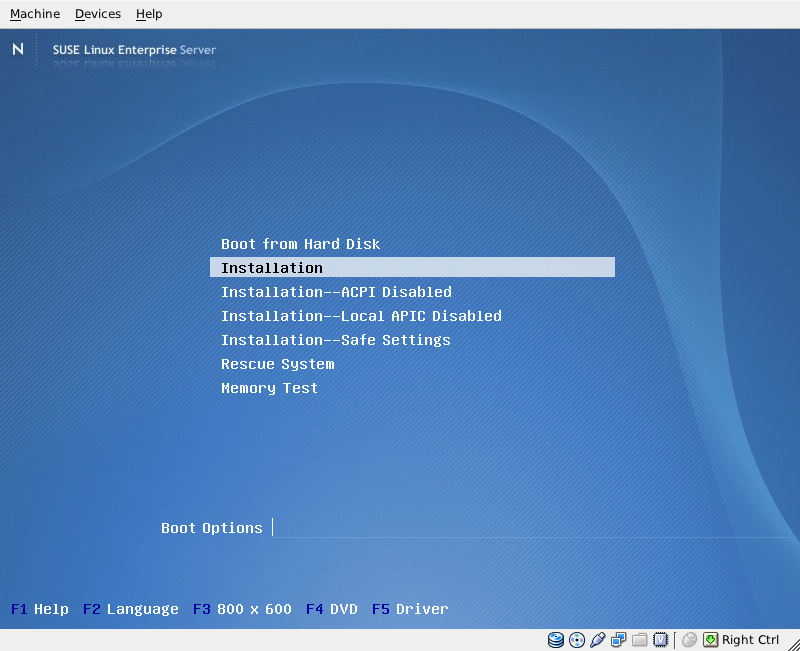
\includegraphics[width=1\linewidth]{oes/1.png}}
\caption{Начало установки}
\label{fig1}
\end{figure}
По умолчанию выбран пункт «Boot from Hard Disk» (Загрузка с жёсткого диска). Для начала установки выбираем пункт «Installation».\\

Первое окно — выбор языка установки, выбираем <<Русский>>, нажимаем next. (рис.~\ref{fig2})
\begin{figure}[H]
\center{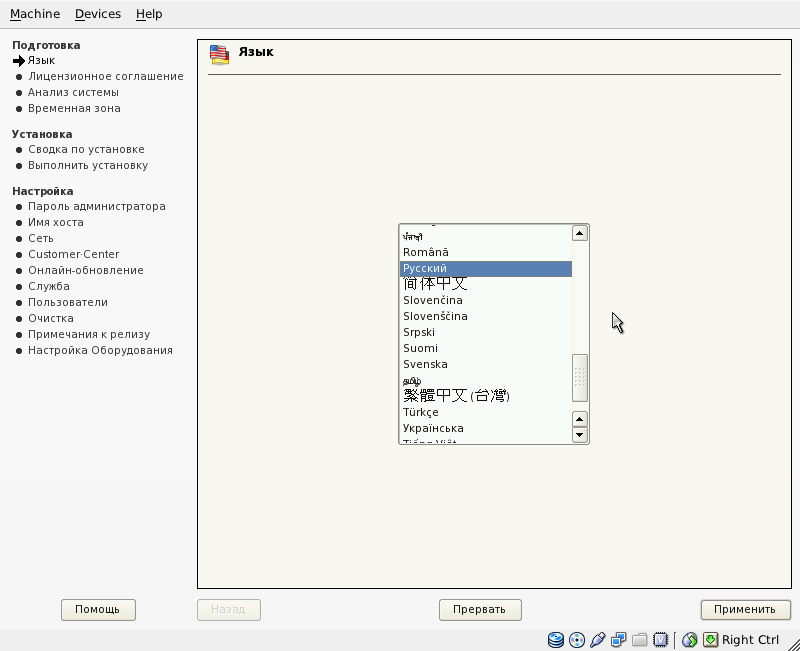
\includegraphics[width=1\linewidth]{oes/2.png}}
\caption{Выбор языка}
\label{fig2}
\end{figure}

Далее предлагается принять лицензию на SLES10 «Да, я согласен с условиями лицензионного соглашения>>, без чего дальнейшая установка невозможна. (рис.~\ref{fig3})
\begin{figure}[H]
\center{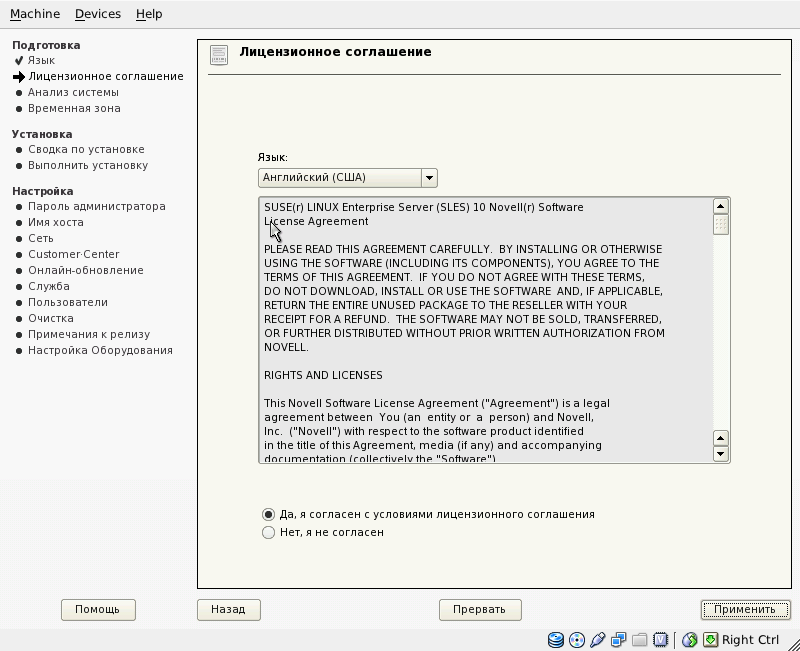
\includegraphics[width=1\linewidth]{oes/3.png}}
\caption{Лицензионное соглашение}
\label{fig3}
\end{figure}

\section{Настройка}
Настройка сети. Нажимаем <<Изменить>> -> "Сетевые интерфейсы", "Установка статического IP адреса" 192.168.0.2\\
"Имя хоста и сервер имён" -> Прописываем наш сервер в "Сервер имён 1" жмём "Применить"\\

Управление сертификатами. <<Управление СА>> -> "Редактировать Установки по Умолчанию" -> Страна: Россия\\


\subsection{Шаг 1}
Поднимаем Active Directory (Или что там вместо него).

\subsection{Шаг 2}
Что-нибудь еще\ldots